% Copyright (c) 2014,2016 Casper Ti. Vector
% Public domain.

\chapter{面向人工智能的云计算系统软件研究}
% \pkuthssffaq % 中文测试文字。
以深度学习为代表性技术的人工智能领域在21世纪10年代再度兴起,社会各界对于人工智能的需求也愈发旺盛。遍布超市和餐馆中的扫脸支付技术、智能手机上的语音智能助手、工厂中检测废件的自动检测装置等,都离不开人工智能技术的加持。上述场景都需要适当的机器学习模型在线部署以提供服务。

机器学习的工作流一般遵循如下几个步骤:1)模型开发与调试。在此阶段中,开发者根据具体的场景,编写并调试模型代码。2)模型参数调整。在这个步骤中,开发者使用训练集不断调整模型的超参数,使其在测试集上的表现符合某种标准(如准确率高于某个阈值)。3)模型部署,开发者将开发完成的模型部署到对应的场景中对外提供服务。

为了方便开发者专注到模型的开发流程中,各大主流云厂商均实现了支持机器学习模型开发-调试-部署整个流程的软件栈。同时,云厂商提供的一般性的平台可能无法满足用户特定的需求。因此针对具体场景,学术界也提出了一系列基于云服务的机器学习软件,以达到降低开发成本、提高模型在线服务的质量等目标。本章对上述内容涉及到的相关工作展开具体研究。

\section{公有云厂商提供的云上机器学习系统}

本节先介绍公有云厂商机器学习系统所遵循的共同范式,即Parameter Server系统架构。再以AWS Sagemaker为代表,介绍公有云厂商一站式的云上机器学习系统的设计。其它厂商中类似系统中对计算模型的抽象、使用方式等均与Sagemaker大同小异。

\subsection{Parameter Server架构}
大模型的训练一般难以在单机上运行,需要分布式的环境将更多的算力和存储资源组织起来。A. Smola等人\parencite{smola2010an}在2010年为了解决大型自然语言处理模型的训练,提出来一种并行的分布式训练架构。在该架构中,模型的参数通过key-value的形式存储在一部分节点上,另一部分节点负责训练,同时在完成训练后将参数push到存储参数的节点上。该架构实际上就是后来业界流行的Parameter Server架构,即参数服务器架构(简称为PS Model),的雏形。

此后类似的架构在产业界得到了广泛使用。直到2014年,M. Li等人\parencite{186214}在OSDI上发表论文,综合地描述了PS Model的设计和实现,并完善了PS Model的通信模型、参数同步和异步的push/pull模型、server节点的一致性模型。至此,PS Model实际上已经开始逐渐成为业界大型分布式机器学习系统的设计范式。

如图~\ref{ps_arch}所示,在一个基于PS Model的集群中,服务器被分为两种,分别为worker和server。其中server负责保存模型所有需要训练的参数,worker负责具体的训练。在worker完成一轮迭代之后,会将更新后的参数变化量push到server端,并同步等待所有其它的worker完成此轮迭代。同步完成后,server汇总从worker端得到的变化量并对参数进行更新,而后worker再从server端pull更新后的参数,并继续进行下一轮迭代。值得一提的是,实际场景中为了追求训练速度,有时也会允许异步的参数更新,即不要求worker等待其它peer节点完成本轮计算,而是完成本地计算后就可以向server请求pull新的参数。这种弱一致性的设计会加快训练速度,通过也可能牺牲模型的质量。

\begin{figure}[h]
    \centerline{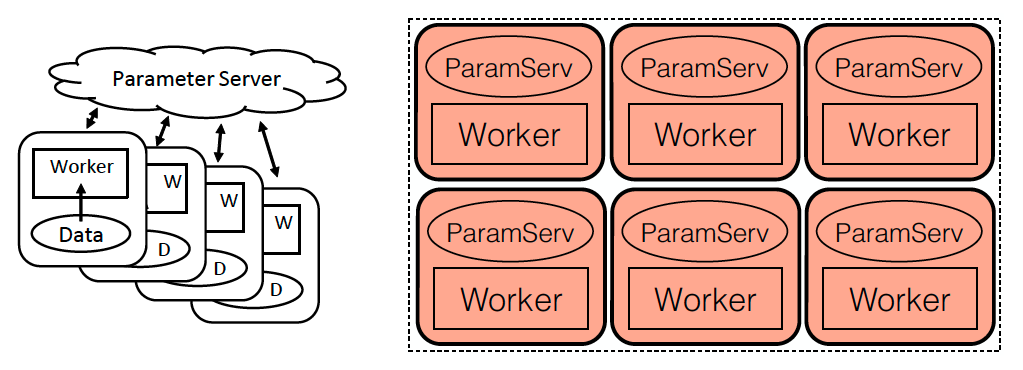
\includegraphics[width=\textwidth]{figures/ps-arch.png}}
    \caption{参数服务器系统架构。}
    \label{ps_arch}
\end{figure}

PS Model之所以能够高效,与其worker push和pull参数时的设计是密切相关的。 图~\ref{ps_sgd}阐述了在PS Model中使用梯度下降训练模型时的流程。值得注意的是,生产环境中的数据集一般都是稀疏的。例如用户画像数据,每个用户几乎不可能将所有表示其特征的列填满,很大概率会空余一些特征。如图中所示,每个worker被分配到的数据所对应的特征实际上只是整体数据集特征的一个子集。因此,在PS Model中,每个worker只会计算本地特征对应的参数增量,并这部分参数push到server节点上。在本轮结束后,再从server节点pull本地需要的参数。这种场景下,key-value形式的参数存储就体现出了优势。每个worker通过key指定自己需要的参数,从而大大降低了节点之间的数据传输量。

\begin{figure}[h]
    \centerline{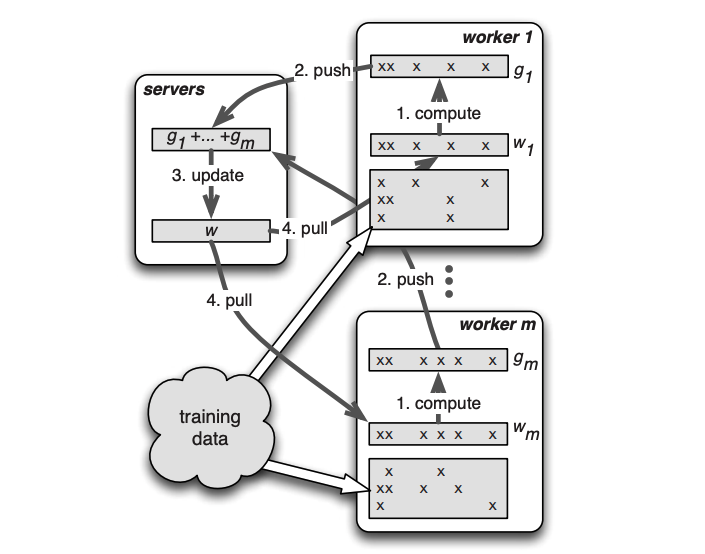
\includegraphics[width=\textwidth]{figures/ps-sgd.png}}
    \caption{在参数服务器架构中使用梯度下降训练模型的流程。}
    \label{ps_sgd}
\end{figure}

\subsection{AWS Sagemaker}\label{subsec_sagemaker}
AWS作为公有云领域的先驱者,在云计算的前沿技术领域一直处于领先的地位。其某些代表性技术甚至成为了多数公有云厂商所共识的标杆和规范。在机器学习系统这一分领域,其代表性系统为AWS Sagemaker。

Sagemaker是一个实现和产品化机器学习模型的框架\parencite{joshi2020amazon},用户可以将其模型训练需要的数据存储到AWS的对象存储服务S3中。然后,用户可以通过web的方式访问部署在云端的Jupyter Notebook服务,在线访问数据、编写并调试代码。当模型训练完毕后,可以使用Sagamaker内置的推理服务对模型进行发布。用户在发布时还可以根据平台的不同(云端或边缘节点)将模型打包编译成不同的版本。此外,Sagamaker还内置了一些常用的算法和数据集,方便开发者直接调用。

在训练算法和系统机制方面,Sagemaker旨在解决工业规模的模型训练场景中的如下几个常见问题:

\begin{itemize}
    \item \textbf{支持增量式的训练和模型更新。}在真实的工业场景中,几乎不存在完全静态的数据集。用来训练模型的数据集大多都是不断增长的。例如电商网站的用户行为数据,每天都在以相当的速度增长。在这样的动态数据上训练模型,势必要进行如下权衡:在全量数据上进行训练,可以获得质量更高的模型,然而时间和经济上的开销却会非常高;在最新更新的数据上(例如最近几天的数据)进行训练,可以快速的得到新的模型,却有可能在一定程度上牺牲模型的准确性。
    \item \textbf{容易估算训练模型产生的花销。}对于体量非常大的数据集,用户需要较为准确地估计训练模型将会产生的时间和经济花销。当今的云计算一般遵循按量付费的收费模式,因此云上的机器学习用户会格外关注花销的问题。
    \item \textbf{支持暂停和恢复模型训练,有一定的弹性。}生产环境中,大模型的训练通常包含跨越数十甚至上百台机器的并发任务。在一些场景中,由于超参数调整的需要或者计算资源的限制,开发者需要对这些任务进行中断和恢复。这就要求云上的ML系统能够支持大型训练任务中断和恢复时中间结果的保存和复原。
    \item \textbf{能够处理非持久性数据。}在很多场景中,数据并不一定是持久化的,也会有很多“瞬时”的数据,例如直播时的视频流等。这些数据一般不会被持久化保存,因此如何支持对这些数据的挖掘和学习也是一个重要的问题。
    \item \textbf{支持自动调参。}自动调参是一项非常耗时耗力的工作,特别是在生产环境的大数据集下。因此,如何能够支持高效的自动调参,方便用户选取合适的模型,对于云上的ML系统而言也是非常重要的。
\end{itemize}

下面将从计算模型、支持算法和具体的实现方式介绍Sagemaker如何解决上述问题。

\subsubsection{计算模型}
Sagemaker将机器学习训练的工作流抽象为三个阶段:initialize,update和finalize。initialize阶段:对相关的变量进行初始化。update阶段:系统以数据流及其状态作为输入,根据用户编写算法更新状态。在Sagemaker的后台,状态更新是在多台计算节点上同步执行的。finalize阶段:对之前所有的更新进行汇总,并输出最后的结果(对于机器学习任务而言,一般是一个模型)。通过上述抽象,用户只需编写initialize、update和finalize三个函数,就可以将整个训练过程交由Sagemaker,等待最后的模型输出。

算法~\ref{algo_sagemaker}用伪代码的形式讲述了三个阶段的具体流程。这里以计算一列数据的中位数为例,使用随机梯度下降(SGD)进行求解。对于如下一列数据:$x_1, x_2, x_3, ..., x_n$,则由如下公式给出这一列数据的中位数:$\operatorname{argmin}_z\Sigma_{i=1}^n||x_i-z||$。算法中的initialize函数首先对median和n两个参数做初始化。这里\textit{state}可以理解为一个key-value存储结构。在update阶段,函数将接收到的数据流\textit{data\_stream}分为若干mini\_batch,对每个batch没的数据,迭代式的对median值进行更新,同时更新n的值。最后,在finalize函数中,对最终的median值进行汇总。同时,系统还支持用户在算法的任意位置设置barrier(第15行),以对整个训练过程进行同步操作。

\begin{algorithm}
    \caption{Sagemaker计算模型}
    \label{algo_sagemaker}
    \begin{algorithmic}[1] 
        \Function{initialize}{$state$}
        \State $state.initialize('median', 0)$
        \State $state.initialize('n', 0)$
        \EndFunction
        \State
        \Function{update}{$state, data\_stream, synchronized$}
        \For {$mini\_batch \in data\_stream$}
        \State $current\_median \gets state.pull('median')$
        \State $n \gets state.pull('n')$
        \State $inc \gets 0$
        \State $batch\_size \gets 0$
        \For {$item \in mini\_batch$}
        \If {$item > current\_median$}
        \State $inc += 1$
        \Else
        \State $inc -= 1$
        \EndIf
        \EndFor
        \State $state.push('n', batch\_size)$
        \State $state.push('median',\frac{inc}{\sqrt{n + batch\_size}})$
        \If {$synchronized$}
        \State $state.barrier()$
        \EndIf
        \EndFor
        \EndFunction
        \State
        \Function{finalize}{$state$}
        \State \Return{$state.pull('median')$}
        \EndFunction
    \end{algorithmic}
\end{algorithm}

\subsubsection{支持算法}
尽管深度学习在近年越来越流行,特别是在学术界,各种刷新SOTA(即state-of-the-art,当前最优)效果的模型层出不穷。然而在产业界,经典的机器学习模型适用性依然非常广。本节对Sagemaker支持的广泛应用于产业界的经典机器学习模型做简单介绍。

\textbf{Linear Learner. }即线性回归模型,一般用来解决回归或者分类问题。在Sagemaker中,其支持使用随即梯度下降(SGD)来训练一个线性模型。特别地,Sagemaker还支持对一个模型指定不同的目标函数,并且并行地训练其对应的多个模型。

\textbf{Factorization Machines (FM)\parencite{rendle2010factorization}. }FM常用于推荐系统中很多任务(例如CTR预估),是一种适用于分类和回归任务的更为通用的监督学习算法。FM是对线性模型的一种拓展,考虑了高维稀疏数据集中不同特征之间的关联。在Sagemaker中,FM也是通过SGD来进行训练的。

\textbf{K-Means Clustering\parencite{jain2010data}. }K-Means聚类是一类无监督学习算法,可以将一个数据集聚为K个不同的类别。Sagemaker实现了一个流式计算版本的K-means,综合运用了来自随机优化、核心集和在线选址问题的思想。

\textbf{Principal Component Analysis (PCA).\parencite{tenenbaum2000a} }即主成分分析,是一种通过尽可能保留数据集的方差来对数据进行降维的算法。Sagemaker实现了两种PCA算法。第一类是准确型的,通过适量的采样和特征提取,需要$O(d^2)$量级的内存大小。另一种是粗略型的,通过随即投影来减小内存开销到$O(kd)$。这里$k$和$d$分别代表主成分的个数和数据的维度。

\textbf{Neural Topic Models (NTM). }在Sagemaker中,NTM是一种用来在大型离散数据集中抽取latent representation的无监督学习算法,例如抽取文档中的语料库。为了实现更快的推理,NTM是基于variational autoencoder(VAE)模型实现的。

\textbf{Time Series Forecasting with DeepAR. }这是一种基于循环神经网络(RNN)的概率预测算法。和其它流行的时间序列预测算法不同,DeepAR\parencite{flunkert2020deepar}使用一系列数据集训练了一个全局的模型,从而重点关注了在生产环境中常见的时间序列预测问题。

\subsubsection{实现方式}
经济和高效是云用户总是在关心的两类问题。Sagemaker为了满足这样的用户需求,充分利用了其底层的异构资源池,并通过上层的系统软件使得机器学习可以在成百上千台VM上横向拓展。

\textbf{在异构硬件上运行ML任务。}
为了实现在异构的资源上(主要是CPU和GPU),Sagemaker中的大多数算法使用MXNet\parencite{chen2015mxnet}的库作为使用底层硬件的接口。MXNet通过一个张量算子构成的计算图来描述一个机器学习算法,同时通过将算子分配到具体的设备进行执行来实现并发地训练模型。

\textbf{利用参数服务器模型(Parameter-Server Model,即PS Model)\parencite{186214}实现分布式训练和参数共享。}如图~\ref{sagemaker_ps}所示,在Sagemaker中,分布式训练就是通过参数服务器模型来实现的,且一般默认使用的是弱一致性的模式。同时,为了方便push和pull的操作,AWS实现了一个key-value的存储系统KVStore。

\begin{figure}[h]
    \centerline{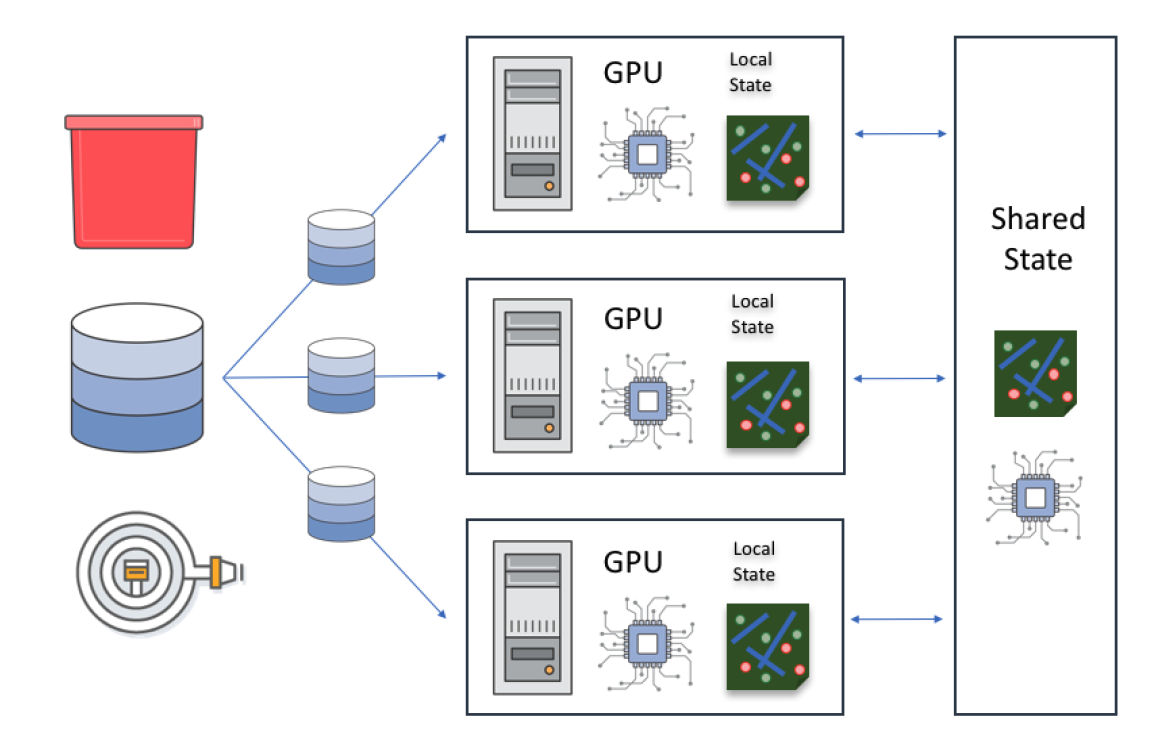
\includegraphics[width=\textwidth]{figures/sagemaker-ps.png}}
    \caption{基于PS Model的Sagemaker系统架构。}
    \label{sagemaker_ps}
\end{figure}

\textbf{模型抽象与参数表达。}Sagemaker在上层为用户提供了模型抽象和参数的表示方式。对于一个模型而言,有两个与其绑定的函数需要用户来实现:1)\textit{score}函数,为一个模型打分以衡量模型在该数据集的训练程度,在调试或者超参数调整阶段会被用到;2)\textit{evaluate}函数,接受一个batch的数据并计算该模型的输出。需要指明的是,对于不同的模型而言,输出的格式可能是不同的,例如对于分类问题,输出可能是一个label也可能是不同类别的概率。参数的表达方式同样需要统一的上层抽象。在Sagemaker中,不同类型的模型有着不同的表达形式。例如,K-means算法的模型就表现为一个核心集,因此,对于任意$k<k_{max}$,用户都无需重新训练模型,而是可以直接得到结果。对于K邻近算法,Sagemaker也有类似的设计。

\begin{figure}[h]
    \centerline{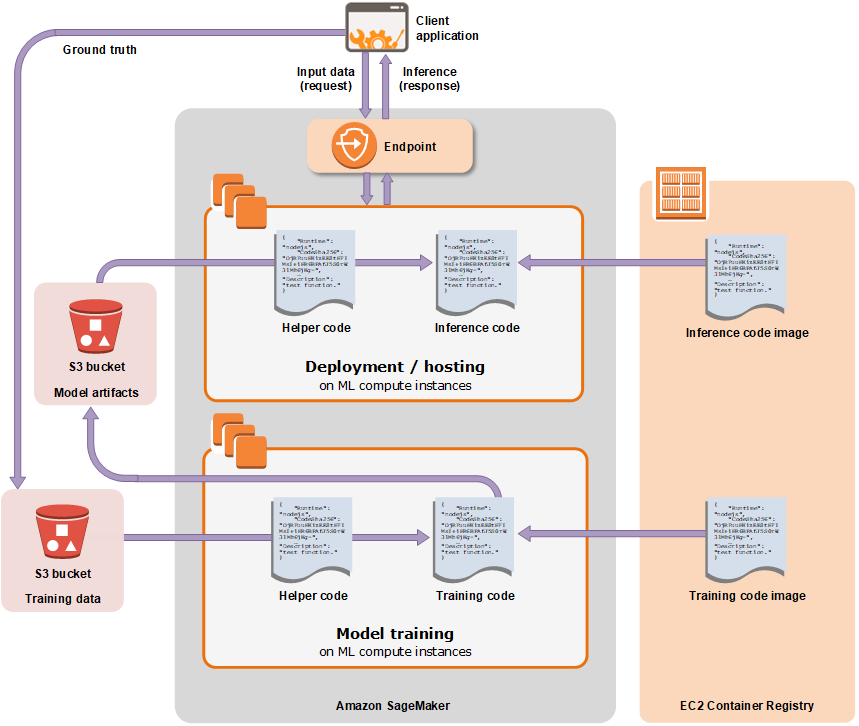
\includegraphics[width=\textwidth]{figures/sagemaker-architecture.png}}
    \caption{Sagemaker训练、部署工作流。}
    \label{sagemaker_train_serving}
\end{figure}

\textbf{模型微调与超参数调整。}通常而言,一个超参数调整任务(Hyperparameter Tuning Optimization,即HPO)\parencite{bardenet2013collaborative}由多个并行的模型训练任务构成,这些训练任务每个都尝试一个不同的超参数组合,最后得到一个最优的配置。上述过程需要耗费大量计算资源和时间,对于寻常用户而言是非常耗时耗力的。而Sagemaker基于PS的计算模型设计保证了任意一个ML训练任务都可以随时启动和停止。这种机制使得模型微调和超参数调整变得更为容易操作:1)用户可以增量式地更新数据集,但却不用每次都重新训练模型,因为整个训练过程都是流式的;2)HPO可以同时启动多个训练任务,然后提前发现那些劣质的模型并将其终止,从而降低HPO的成本。

\subsubsection{模型部署}
作为一站式的机器学习系统,除了模型训练和调参,Sagemaker还支持模型部署。图~\ref{sagemaker_train_serving}展示了Sagemaker训练和部署模型的整体工作流。在部署时,首先,用户需要对其模型指定一个endpoint,然后将部署该模型的的代码打包成容器镜像,存储在EC2 Container Registry中。在模型实际对外提供服务时,模型文件会从对象存储S3中传输到容器中,进而以容器为单位对外提供服务。

\section{基于公有云服务的第三方机器学习系统}
尽管公有云厂商实现了相当完备的一站式机器学习系统,但是随着生产环境中业务场景的日渐复杂,大而全的公有云解决方案已经无法解决个性化的用户需求。例如,某些用户希望以尽可能低的成本完成大型模型的训练,或者在保证模型服务的SLO前提下,能够尽可能低成本的部署机器学习模型。在上述场景中,为了完成用户的具体需求,需要综合利用各类云资源,并制定一定的策略。本节对近几年来几个构建于公有云资源上层的机器学习系统做具体介绍。
\subsection{基于云厂商动态资源的机器学习模型训练系统}
% Proteus by harlap
% SpotTune by Yan
机器学习模型的训练是一个不断在给定数据集上迭代更新参数的过程。对于一些较大的模型,训练时间一般会非常长。特别是深度神经网络模型再度兴起后,模型开始变得越来越庞大。例如Open AI的自然语言模型GPT-3,包含1750亿个参数,单单存储这些参数就需要450GB的空间。而训练该模型的成本,据估计更是达到了1200万美元。对于一些个人开发者和小型公司,大模型的训练往往显得遥不可及。

除了上述可训练的参数之外,还存在大量不可训练的参数。例如,SVM模型中核函数的类型,树模型中树的深度,深度神经网络模型中网络的宽度和深度等。这些参数需要由开发者在训练之前事先决定,一般被称为超参数。不同的参数组合在一起,就构成了巨大的搜索空间。例如,如果存在6个超参数,每个超参数有4种不同的选择,就会产生$4^6=4096$种不同的超参数组合。

完全遍历所有的超参数组合是非常费时费力的,通常情况下也是不切实际的。研究者为了减少超参数搜索的此时,提出了诸如网格搜索、贝叶斯搜索等技术。但即便如此,仍然需要大量的算力来支撑整个搜索过程。

而与此同时,在云计算时代,云上资源的易用性、高度的弹性以及收费模式的多样性使得以较低的成本完成费时费力的模型训练和超参数搜索变为可能。如上一小节所述,一些云厂商提供了一些价格低廉的动态资源。和一般的可以获得可用性保障的资源相比,这类资源拥有相同的计算能力,但是可用性比较低,在某些场合会被云厂商主动回收。基于上述事实,可以形成一个直观的想法:在这类廉价的资源上运行机器学习模型训练和调参任务,并辅以一定的容错策略和资源选择策略,可以显著降低成本。

\begin{figure}[h]
    \centerline{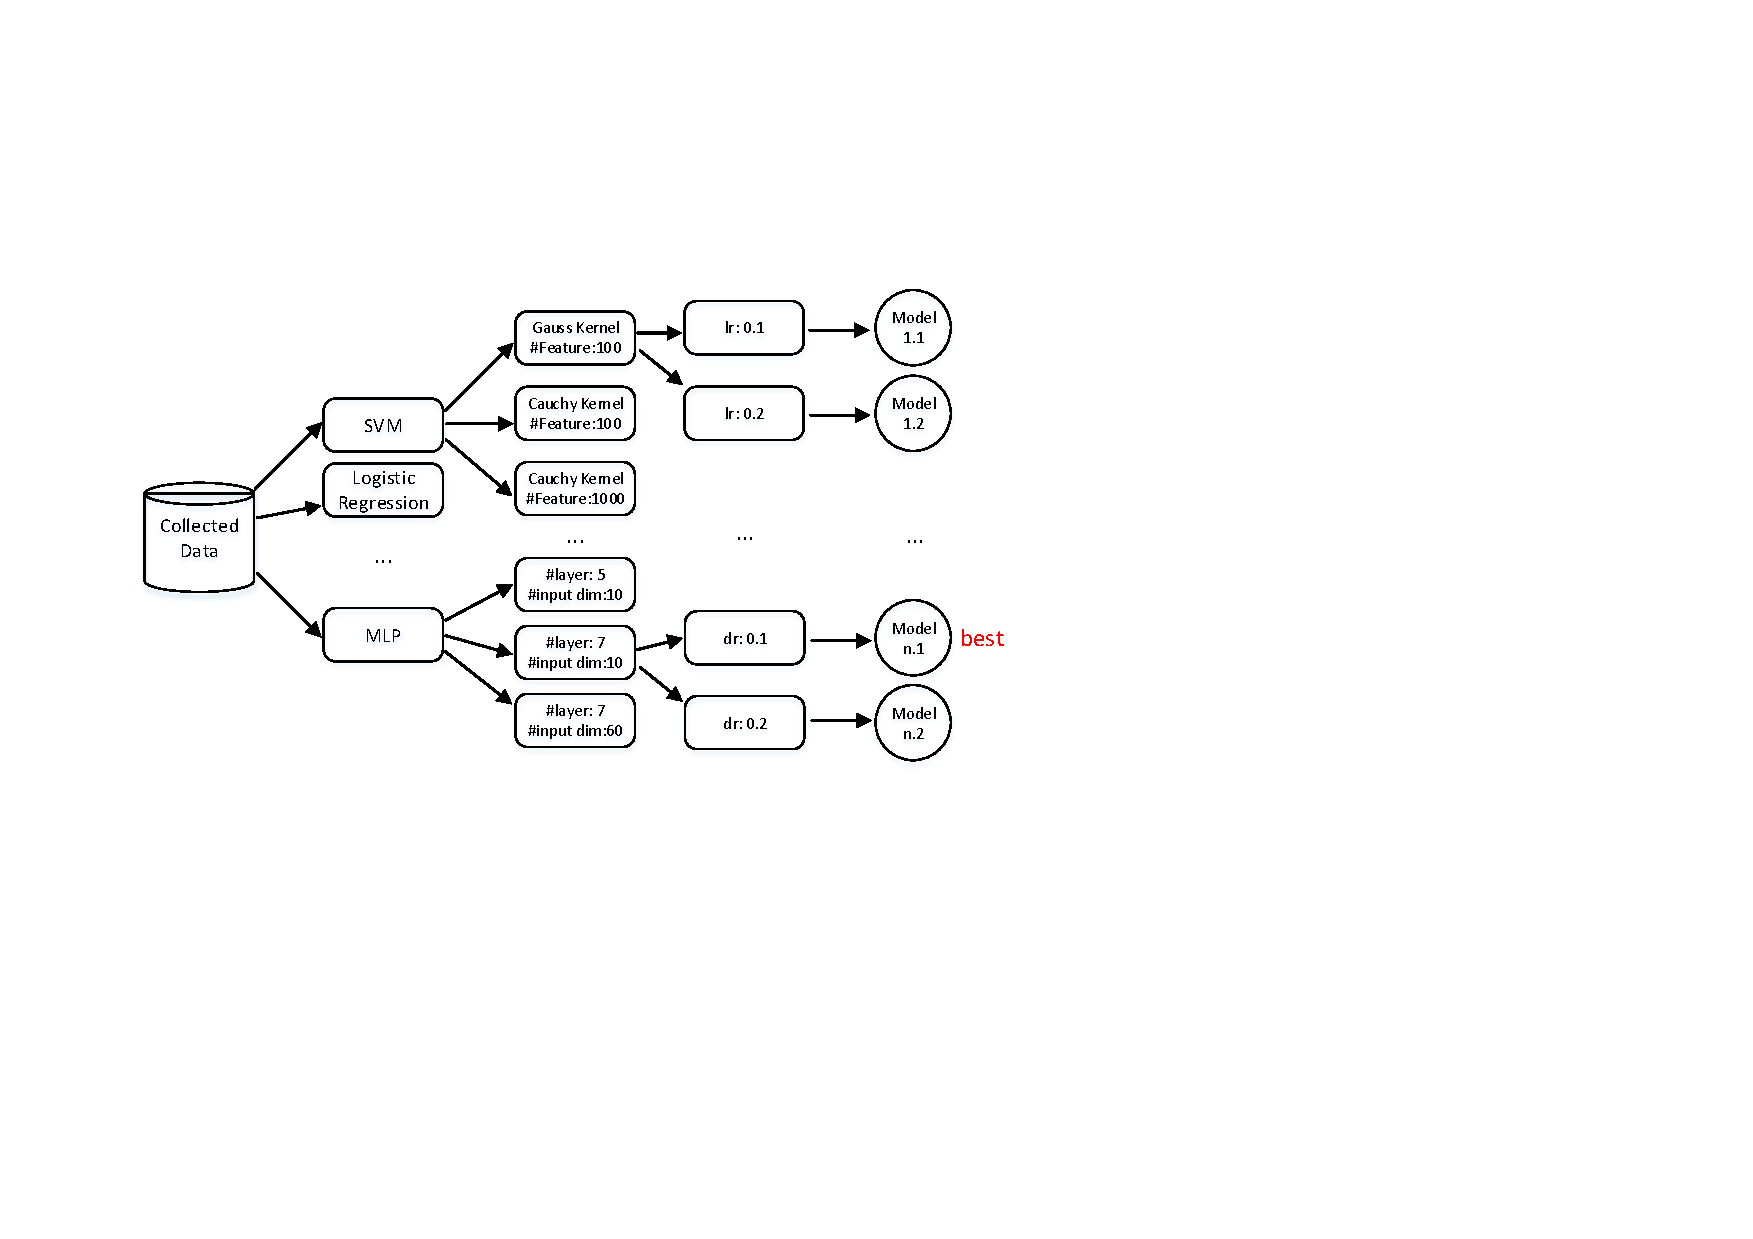
\includegraphics[width=\textwidth]{figures/hpt.pdf}}
    \caption{一个超参数调整的例子。}
    \label{hpt_example}
\end{figure}

但是,在动态资源上运行机器学习模型训练和调参,虽然直觉上会降低成本,但是可能会产生额外的风险。因此,要做到高效并可靠地在动态资源上运行上述作业,还有如下若干问题需要解决:

\textbf{1. 及时处理中断。}动态资源之所以廉价,是因为其稳定性比较低。通常情况下,在某些特殊情况下(例如集群中的负载比较高,需要动态资源来补充资源池),云厂商有权利主动回收这些动态资源。如果不处理这种回收引起的中断,机器学习模型的训练就要被动终止。因此需要采取一些手段,例如提前保存模型或者迁移任务,以及时处理中断。

\textbf{2. 合理的资源选取算法。}事实上,这是在云上运行任务时需要考虑的一个通用问题。用户在云上运行作业时,一般会有一个目标,例如作业运行时间最短或者最终的总体成本最低。因此需要通过一定的算法,为用户选取能满足其需求的资源。对于机器学习模型训练与调参任务亦是如此。

\textbf{3. 充分利用云的弹性。}事实上,在机器学习模型训练过程中,存在大量的无效计算。如图~\ref{hpt_example}所示,经过大量的参数尝试,最终只剩余一个有效模型(即效果最好的模型)。因此,在参数搜索的过程中,大量的计算是无效计算。而云计算的一个重要特点就是高弹性,即用户可以因为负载增加随时获取资源,也可以因为资源闲置随时释放资源。如果效果不好的模型能够被提前发现,并释放掉其占用的计算资源,则可以避免大量无效计算,从而进一步节省成本。

\textbf{4. 对计算框架进行定制。}现有的流行的机器学习框架如Tensorflow\parencite{abadi2016tensorflow},PyTorch\parencite{paszke2019pytorch},MXnet\parencite{chen2015mxnet}等,一般都假设底层的计算资源是可靠的,因此都没有针对上述动态资源进行适配。如果要在动态资源上运行ML任务,则需要对框架进行深度定制,使其具备一定的容错能力。

为了解决上述问题,使ML模型训练和调参都可以在云上经济高效地进行,许多研究者提出了若干解决方案。A. Harlap等人在2017年提出了ML模型训练系统Proteus\parencite{harlap2017proteus},针对Parameter Server架构的ML模型训练框架对AWS和Google Cloud的动态资源做了适配,使其能高效经济地在之上运行。Y. Peng等人在2018年提出基于PS Model的深度学习集群调度器Optimus\parencite{peng2018optimus},通过动态调整集群中PS Model的server和worker的数量比例,并结合对任务完成时间的预测,使集群的吞吐率最大化。Y. Li等人在2020年提出了SpotTune\parencite{li2020spottune},将ML调参任务部署在AWS动态资源上,并结合一定的资源选取算法和训练趋势预测算法,使调参任务节省大量的无效计算,最终达到了经济高效的目的。下文对较有代表性的Proteus和SpotTune做较为详细的介绍。

在介绍相关系统之前,有必要对目前云市场上常见的资源类型、本节重点研究的动态资源及其收费模式做简要介绍。

云计算作为互联网时代下的一种新型计算模式,通过虚拟化和软件定义技术将服务器、存储、网络甚至软件等各种资源聚集为共享资源池。这些虚拟资源用则进行分配,而且种类和数量均可按需配置并按实际用量计费,不用则回收到资源池中等待下次分配。相比传统的IT 资源使用模式,云计算这种按需使用、按量付费的特点增加了用户的灵活性,但也导致了用户需求的不确定性。比如:在销售旺季,用户使用云的频率就会增加,云服务商的负载压力会持续增大甚至超过峰值,进而可能导致故障;而在销售淡季,用户使用云的频率就会大幅下降,云服务商的负荷压力也会大幅降低,导致了空闲资源的浪费。为了充分利用云资源池中的空闲资源,云服务商推出了多种的计费模式,试图以多样化的价格来吸引用户的同时,确保自己在需求高峰时可以回收部分资源。

\begin{table}[!htbp]
    \caption{亚马逊公有云EC2计费模式分析}
    \centering
    \label{tbl_inst_types}
    \begin{tabular}{|c|c|c|c|}
    \hline
    \diagbox{计费模型}{比较}&计费公式&计费特点&适用场景\\
    \hline
    按需实例&\tabincell{c}{实例运行时\\长*单位时\\间对应实例\\费率}&\tabincell{c}{单位时间费率固定,\\无需用户有任何使用\\承诺,价格较高}&\tabincell{c}{适合使用需求周期较\\短、对实例运行环境\\需求多变的用户}\\
    \hline
    预留实例&\tabincell{c}{签约金+$\Sigma$\\第i次运行时\\间*单位时\\间费率}&\tabincell{c}{用户与亚马逊签订长\\时间使用合约,并交\\付签约金,在“合同”\\期内使用EC2 需额外\\支付费用,但费率适\\中}&\tabincell{c}{适合使用需求周期长\\且实例对运行环境性\\能要求稳定的用户}\\
    \hline
    竞价实例&\tabincell{c}{实例运行时\\长*单位时\\间对应实例\\费率}&\tabincell{c}{单位时间实例费率变\\动,根据实例的需求\\情况以拍卖的方式决\\定,费用较低}&\tabincell{c}{适用于没有即时性要\\求、任务可中断的业\\务}\\
    \hline
    \end{tabular}
\end{table}

以亚马逊公有云为例,如表~\ref{tbl_inst_types}所示,EC2 按照计费模式可划分为按需实例(Ondemand Instance)、保留实例(Reserved Instance)和竞价实例(Spot Instance)这三类。相比较于按需实例和保留实例,竞价实例可提供超低折扣,但其价格会随着供需关系而不断调整。用户需要为获取该实例设置一个最高的出价,如果当前市场的价格低于用户的出价,则用户获得实例资源进行计算。一旦市场价格高出用户的出价,则该计算资源会被亚马逊收回。对于公有云厂商来说,竞价实例通过市场机制发掘了云资源的真正价格,达到了其尽可能以最合理的价格卖出最多闲置资源的目标。而对于云平台上的虚拟云用户来说,各种无状态、或者具有容错能力的应用程序可以基于竞价实例来大幅度降低运行成本,代表负载包括:大数据、容器化工作负载、CI/CD、Web 服务器、高性能计算(HPC) 以及其它测试和开发工作负载。尽管竞价实例的出现为非在线业务或者成本敏感业务提供了一种全新的计算资源类型,但是目前来看,无论用户的业务类型为哪种,大部分用户选择的资源依旧是为在线业务所准备的按需实例和保留实例。

竞价实例与按需实例、保留实例的合理使用,可以帮助虚拟云用户优化工作负载的成本和性能。根据AWS 官方博客,已经有不少大型企业(如本田汽车)成功使用AWS 的竞价实例把部分业务的计算成本下降高达70\% 。然而有效的使用竞价实例除了对负载自身的要求以外(如可中断等),还需要用户针对自身的应用场景选择“正确”的实例类型。由于竞价实例在价格和回收方面的不确定性,这是比较复杂的。

Proteus\parencite{harlap2017proteus}是一个基于PS Model架构的机器学习系统。PS是大规模机器学习系统中常用的架构,其系统架构在\ref{subsec_sagemaker}中已描述。如其文中描述,其使用了敏捷的弹性机制并辅以“激进的”竞价策略,使得机器学习任务在云上高效经济地完成。Proteus由两个主要组件构成:AgileML和BidBrain。

其中,AgileML是负责协调整个PS架构的主要组件。其通过如下的基本思想,在保证整个系统可用性的前提下,尽可能多使用动态资源(即AWS Spot Instances)以降低成本:1)将PS的关键功能节点(即保存模型参数的server节点)部署在可靠资源上(如AWS的按需实例或者预留实例);2)将PS的worker节点(即负责实际计算和参数更新的节点)部署在动态资源;3)当动态资源和可靠资源的比例不同时,AgileML会采取不同的策略。具体地,当比例比较小时(例如2:1),其简单地将server节点分布在所有的可靠资源上,而当比例比较大的时候(例如63:1),其将可靠资源作为BackupPSs而将动态资源作为ActivePSs,当发生参数更新时,更新会先到达ActivePSs。同时,在网络带宽允许的前提下,ActivePSs上会启动相应的后台任务将参数同步到BackupPSs上。

\begin{figure}[h]
    \centerline{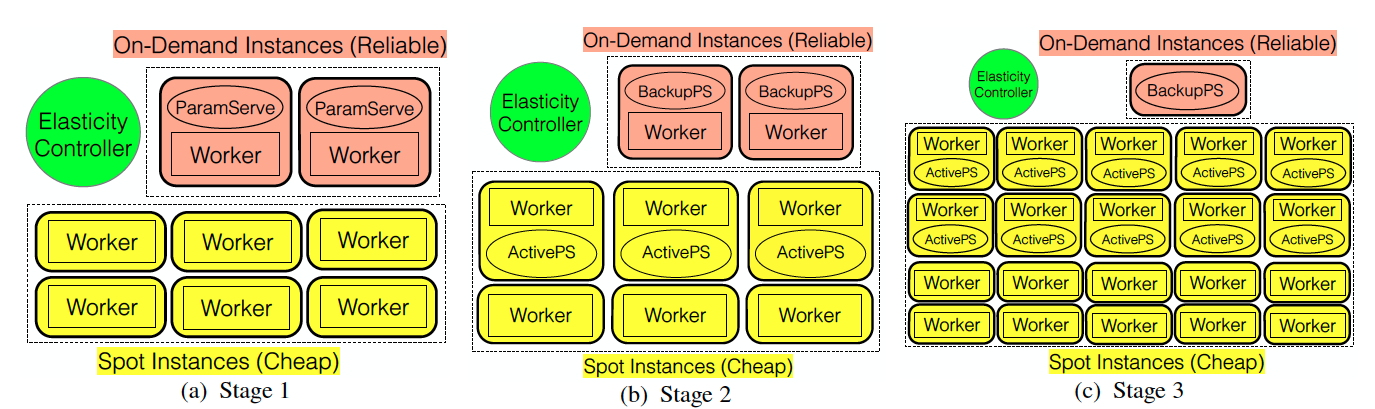
\includegraphics[width=\textwidth]{figures/agileml-stages.png}}
    \caption{AgileML架构中的三个阶段。Stage 1:只存在部署在可靠资源上的ParamServs。Stage 2:ActivePSs部署在动态资源上,BackupPSs部署在可靠资源上。Stage 3:所有的ActivePSs都部署在动态资源上,可靠资源上没有worker。}
    \label{agileml_stages}
\end{figure}

BidBrain是Proteus中的资源管理模块,决定何时获取和释放动态资源。据文中所描述,BidBrain是专为AWS EC2定制的,但是其经过少量的修改和定制化也可以适用于其它环境(如私有集群和其它公有云市场)。其秩序性地监控云市场中动态资源的价格,并即时地竞标那些可能给当前计算带来增益的资源(文中通过 work per dollar来衡量增益,即单位花费可以完成的工作量)。类似地,当一种资源在达到其第一个小时的末端时,就有可能因为性价比降低而被释放掉。另外BidBrain还利用了AWS EC2的一项特殊规则:当资源在其第一个小时内被释放时,其所有花费会被退回。因此其也会主动获取那些在接下来的一小时内会被释放掉的资源,以进一步降低整个成本,此种策略被作者成为激进的竞标策略。总体而言,BidBrain会在激进的竞标策略和保守策略之间权衡,以寻求整个系统的收益最大化。

AgileML的具体功能和技术特点,下文通过一个示例来说明。图~\ref{agileml_stages}描述了AgileML架构中的三个阶段,分别对应不同的资源类型比例。

\textbf{Stage 1:参数服务器仅位于可靠节点上。}此阶段为整个ML训练过程的启动阶段。对于大多数ML的应用程序而言(例如K-means,DNN,Logistic Regression,MF,LDA等),其在PS模型的场景下worker节点是无状态的,其当前轮次更新的参数数据会push到server节点进行持久化存储。因此,在启动时,AgileML会将所有的server节点部署到可靠资源上,而将所有的worker节点部署到动态资源上。在这种情形下,当worker因为云厂商的主动回收而宕机时,整个训练过程并不会受到影响,也不需要进行checkpointing。但是在模式下,当动态资源与可靠资源相比比例过于悬殊时,网络会成为瓶颈。例如当存在60个动态节点和4个可靠节点时,MF的训练速度会下降85%。

\textbf{Stage 2:ActivePSs部署在动态节点上,BackupPSs部署在可靠节点上。}为了解决Stage 1中的网络瓶颈问题,Stage 2中将server节点分为ActivePS和BackupPS两种,其中ActivePS分布在动态资源上,BackupPS分布在可靠资源上。这种策略合理控制了server节点和worker节点的比例,解决了网络的瓶颈问题。所有的参数在ActivePS内部是共享的,并且在后台批量地push到BackupPS上,因此当ActivePS因厂商主动回收而宕机时,BackupPS可以恢复其相关状态,并启动新的动态节点。需要注意的是,在Stage 2中,计算节点,即worker,仍然存在于ActivePS上。

\begin{figure}[h]
    \centerline{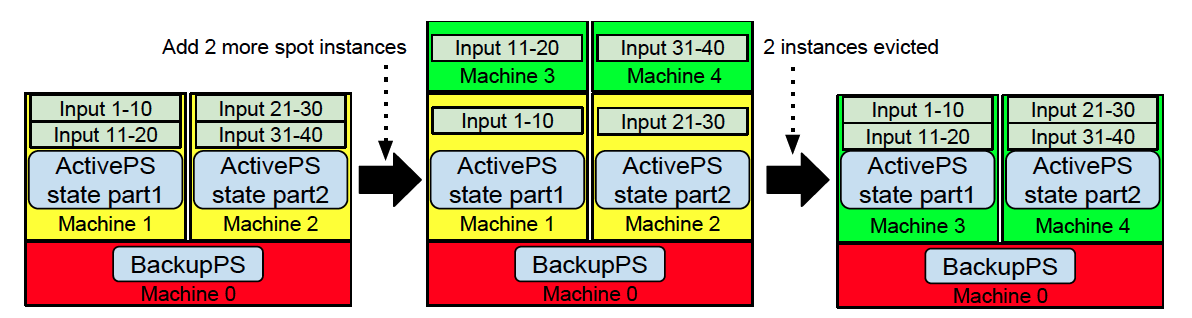
\includegraphics[width=\textwidth]{figures/stage-trans.png}}
    \caption{AgileML动态地添加并删除资源。}
    \label{stage_trans}
\end{figure}

\textbf{Stage 3:所有的计算节点,即worker都位于动态节点上。}实验证明,当动态资源和可靠资源的比例超过15:1时,和BackupPS共同部署的worker会造成“落后者效应”(即Straggler Effect)。因此,Stage 3中简单地移除了所有位于BackupPS中的worker。何时由Stage 2转移到Stage 3,依赖于网络带宽,动态资源和可靠资源地比例以及ML模型的大小等等。

上述三个stage之间的转移一般是由AgileML根据动态资源和可靠资源之间的比例动态决定的。当发生阶段转移时,AgileML会根据实际情况做出相应的动作。例如,当从Stage 1转移到Stage 2时,AgileML会将模型的状态(一般是模型的参数)转移到新增的动态资源上,当动态资源和可靠资源的比例超过一个阈值时,AgileML会将相应的worker在BackupPS上删除,并将相关的训练数据重新分布到其余worker上。图~\ref{stage_trans}所示的是一个stage转移的示例。

BidBrain是Proteus中的资源管理模块,决定何时获取和释放动态资源。其持续性地监控当前和历史的动态资源价格数据,并在相关的时刻根据预测出的花费做出决策,选择当前最优的资源加如动态资源池。简而言之,其资源选取策略较为激进,会考虑那些在未来一个小时就会被回收的Spot Instances,以获取相应的退款,进而进一步降低使用成本。其细节策略与相关的公式推导本文不再赘述。

总体而言,Proteus运用了激进的资源选取策略,将动态资源和可靠资源相结合,进行云上的ML模型训练。经过其实验验证,与仅使用可靠资源相比,Proteus可以实现约85\%的成本节省,和一般的基于checkpoint的云上ML训练系统相比,其效率约可以提升50\%。

与单个模型的训练相比,模型的超参数调整(Hyper-parameter Tuning,下文简称为HPT)在整个ML模型产出周期中位于更上一层。其一般需要开发者尝试模型的多个超参数组合,以得出最优的一个。SpotTune是一个云上自动调参管理系统,通过运用公有云上廉价的动态资源来协调整个HPT过程。据文中所述,SpotTune同样是基于AWS的公有云服务实现的,但是经过一定程度的修改和定制,其可以应用与其它云厂商。为了妥善处理因厂商主动回收产生的中断,SpotTune根据厂商提前发出的通知事先对模型进行checkpoint并将其保存到持久化对象存储中。同时其运用了两个关键技术来保证HPT的经济高效:

\textbf{1. 基于花费的细粒度资源管理。}SpotTune计算花费的粒度非常细。其通过预测动态资源的回收概率和在线对HPT任务进行性能建模,预测出接下来一小时内“单步成本”最低的资源并进行任务部署。

\textbf{2. 基于训练趋势预测的早停机制。}SpotTune将ML模型的训练曲线建模为一个可以预测的、多阶段的函数。简而言之,其可以通过当前时刻收集到的关于模型的质量信息(通常是模型的score函数所得出的结果,例如分类模型的分类准确率,回归模型的平均平方误差等等)来预测该模型在最终收敛时的质量,以提前结束那些劣质模型,节省计算资源。

\begin{figure}[h]
    \centerline{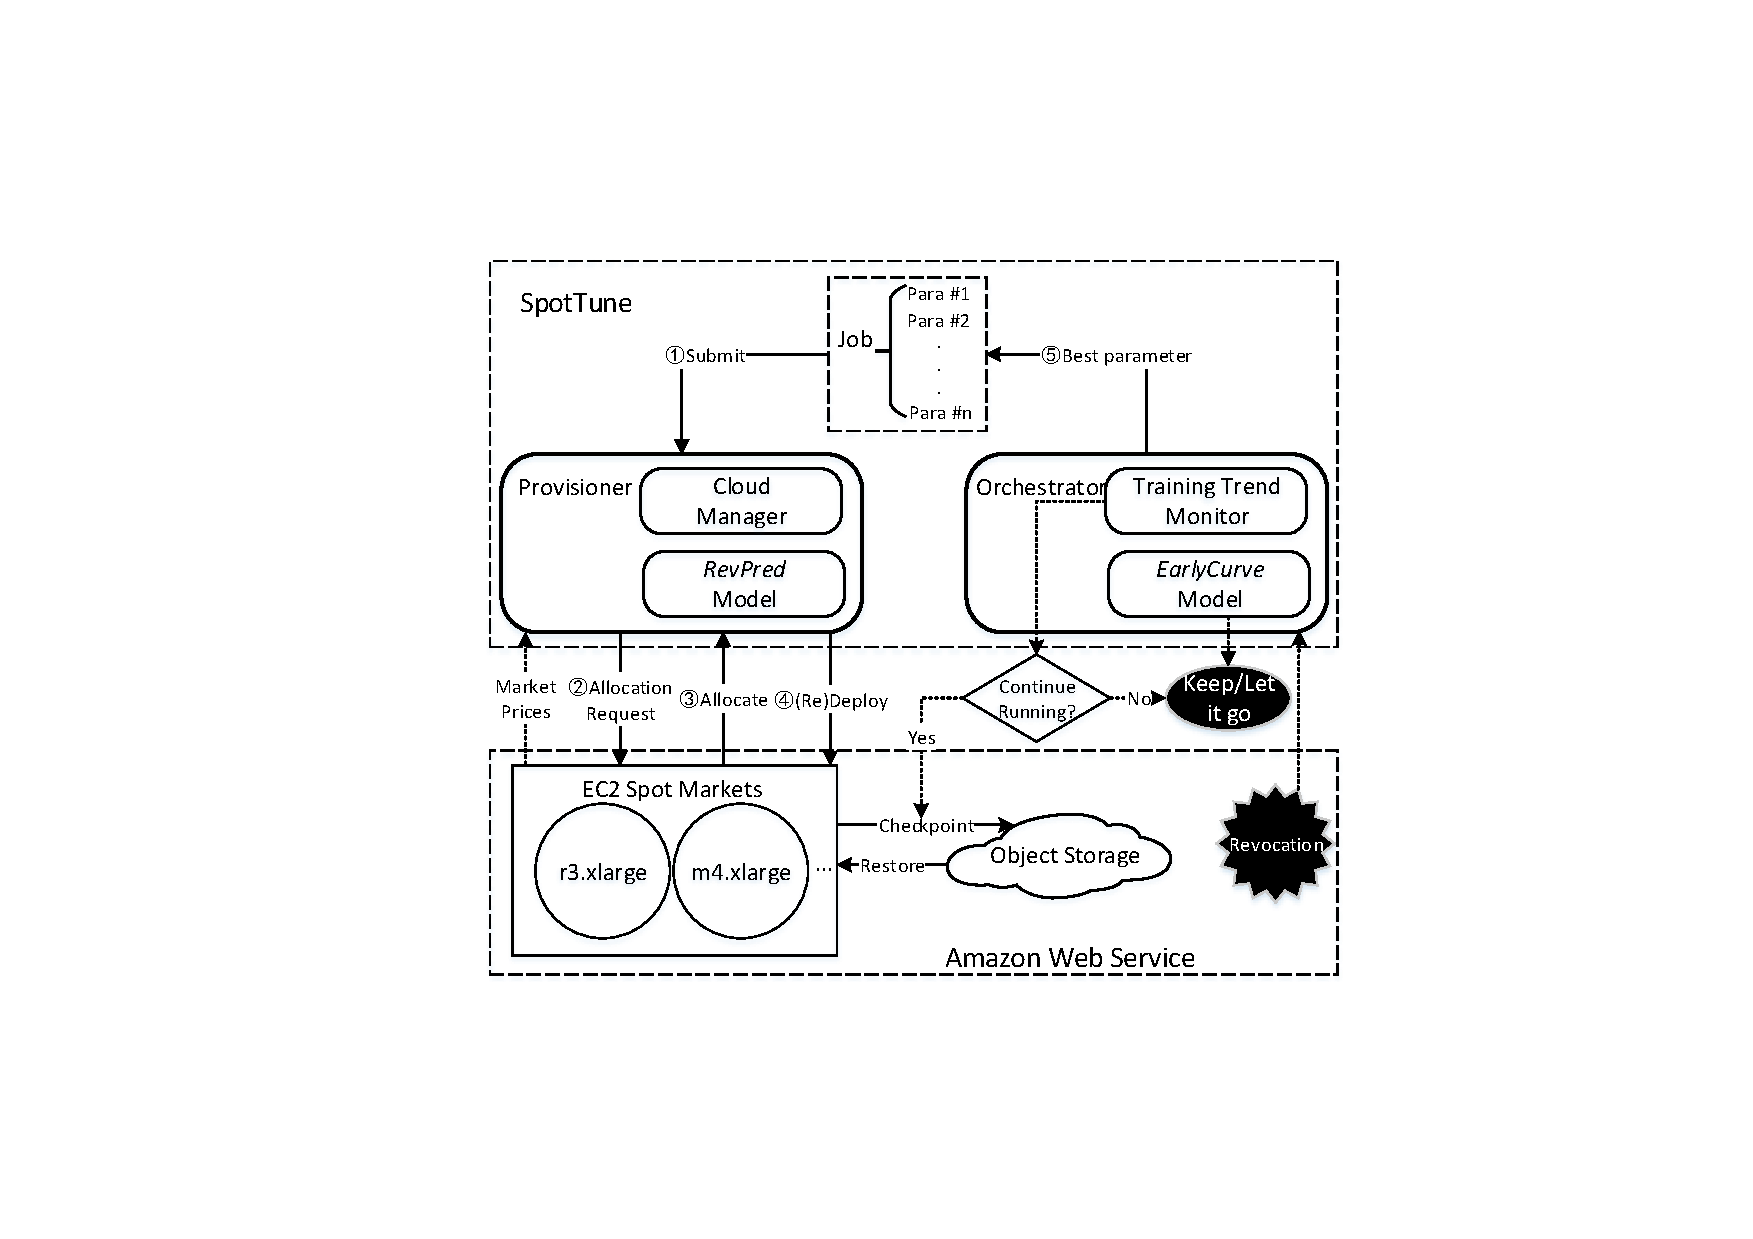
\includegraphics[width=\textwidth]{figures/arch_spottune.pdf}}
    \caption{SpotTune系统架构。}
    \label{arch_spottune}
\end{figure}

SpotTune的系统架构如图~\ref{arch_spottune}所示。其主要功能模块包含Provisioner和Orchestrator两部分。其中\textbf{Provisioner}负责与AWS互动以请求和获取资源。通过结合历史数据和在线更新的性能数据,Provisioner可以细粒度地预测每种资源带来地收益,进而选择最适合HPT任务的资源。\textbf{Orchestrator}负责监控每个超参数组合的训练进度。通过当前收集到的模型质量数据,其可以预测模型的最终质量。Orchestrator一直监听AWS市场的消息,当收到回收提醒时,其会立即将模型checkpoint到持久化存储系统AWS S3中。另一方面,SpotTune认为运行超过一小时的实例性价比是比较低的,在没有特殊情况出现时,Orchestrator会主动将其停止。

SpotTune之所以能做到经济高效,是由Provisioner和Orchestrator中的RevPred模型和EarlyCurve模型决定的。其中RevPred通利用历史数据预测每一种动态资源在将来一小时内被回收的概率,进而用该概率结合在线更新的性能数据预测每一种资源在将来一段时间的效率,其量纲为“\$每步”。具体计算过程如下:

\textbf{1. 计算每种资源在接下来一小时内单价的数学期望。}公式~\ref{eq_ecost}给出了计算方法。公式中的参数$p$为该示例在一小时内被回收的概率。如果该资源被回收(概率对应为p),则价格为零,因为AWS会将该部分费用全数退回给用户。如果该资源没有被回收(对应概率为$1-p$),则按照当前单价收费。

\begin{equation}\label{eq_ecost}
	\begin{aligned}
		\mathbb{E}\left[eCost\right] &= [(1-p) \cdot \overline{price} + p \cdot 0] \cdot 1\ hour \\
		&= (1-p) \cdot \overline{price} \cdot 1\ hour
	\end{aligned}
\end{equation}

\textbf{2. 计算每种资源在接下来一小时内每运行一步(或一个迭代周期,在ML作业中通常体现为一个batch)的花费。}公式~\ref{eq_scost}给出了计算方法。其中$M[inst][hp]$代表了HPT任务$hp$在示例类型$inst$上的运行速度(每步的耗时,seconds / step),由SpotTune持续在线监控模型在每种实例上的训练情况得出。

\begin{equation}\label{eq_scost}
	\begin{aligned}
		\mathbb{E}\left[sCost\right] &= \mathbb{E}\left[\frac{M[inst][hp] \cdot eCost}{1\ hour}\right]  \\
		&=\frac{M[inst][hp] \cdot \mathbb{E}\left[eCost\right]}{1\ hour} \\
		&=\frac{M[inst][hp] \cdot (1-p) \cdot \overline{price} \cdot 1\ hour}{1\ hour} \\
		&=M[inst][hp] \cdot (1-p) \cdot \overline{price}
	\end{aligned}
\end{equation}

至于实例回收概率$p$,SpotTune通过一个精心调试的LSTM神经网络模型来预测,此处不再赘述。

\begin{figure}[h]
    \centerline{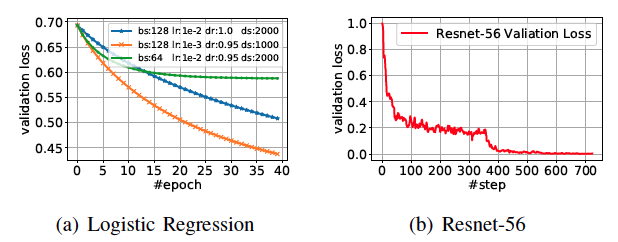
\includegraphics[width=\textwidth]{figures/lr-res56-loss.png}}
    \caption{Logistic Regression与Resnet-56的训练曲线。}
    \label{lr_res56_loss}
\end{figure}


另一方面,SpotTune认为每个ML训练任务的曲线都可以使用一个分段函数进行建模,并利用其部分数据来拟合整个曲线实际的形状,进而预测曲线的最终走势。图~\ref{lr_res56_loss}展示了两种ML任务的训练曲线,都呈现出明显的反比例特征和阶段性特征(通常而言,阶段性的特征一般是由学习率的突变导致的)。且第一张图显示可以通过部分的曲线形状来预测最终的曲线走势,进而提前淘汰一部分模型。EarlyCurve将每个ML训练任务按照公式~\ref{eq_curve_fitting}进行建模,通过当前收集到的部分数据将其拟合为一个分段函数。

\begin{equation}\label{eq_curve_fitting}
	\hat{\mathcal{L}_k} = \sum_{i=1}^{ST}(\frac{1}{\alpha_{i0} \cdot k^2 + \alpha_{i1} \cdot k + \alpha_{i2}} + \alpha_{i3}) \cdot sign(k, l_i, r_i)
\end{equation}

公式~\ref{eq_curve_fitting}工作的前提是用户先指定一个早停系数$\theta \in [0, 1]$,当训练完成$\theta$时,EarlyCurve开始预测模型的最终走势,并在此时淘汰一部分模型。这个参数反映了用户对于调参任务的激进程度,小的$\theta$可能会使预测准确率降低,但是能更快地结束HPT,反之亦然。具体$\theta$的选择,依赖具体场景和用户的具体需求。

\begin{figure}[h]
    \centerline{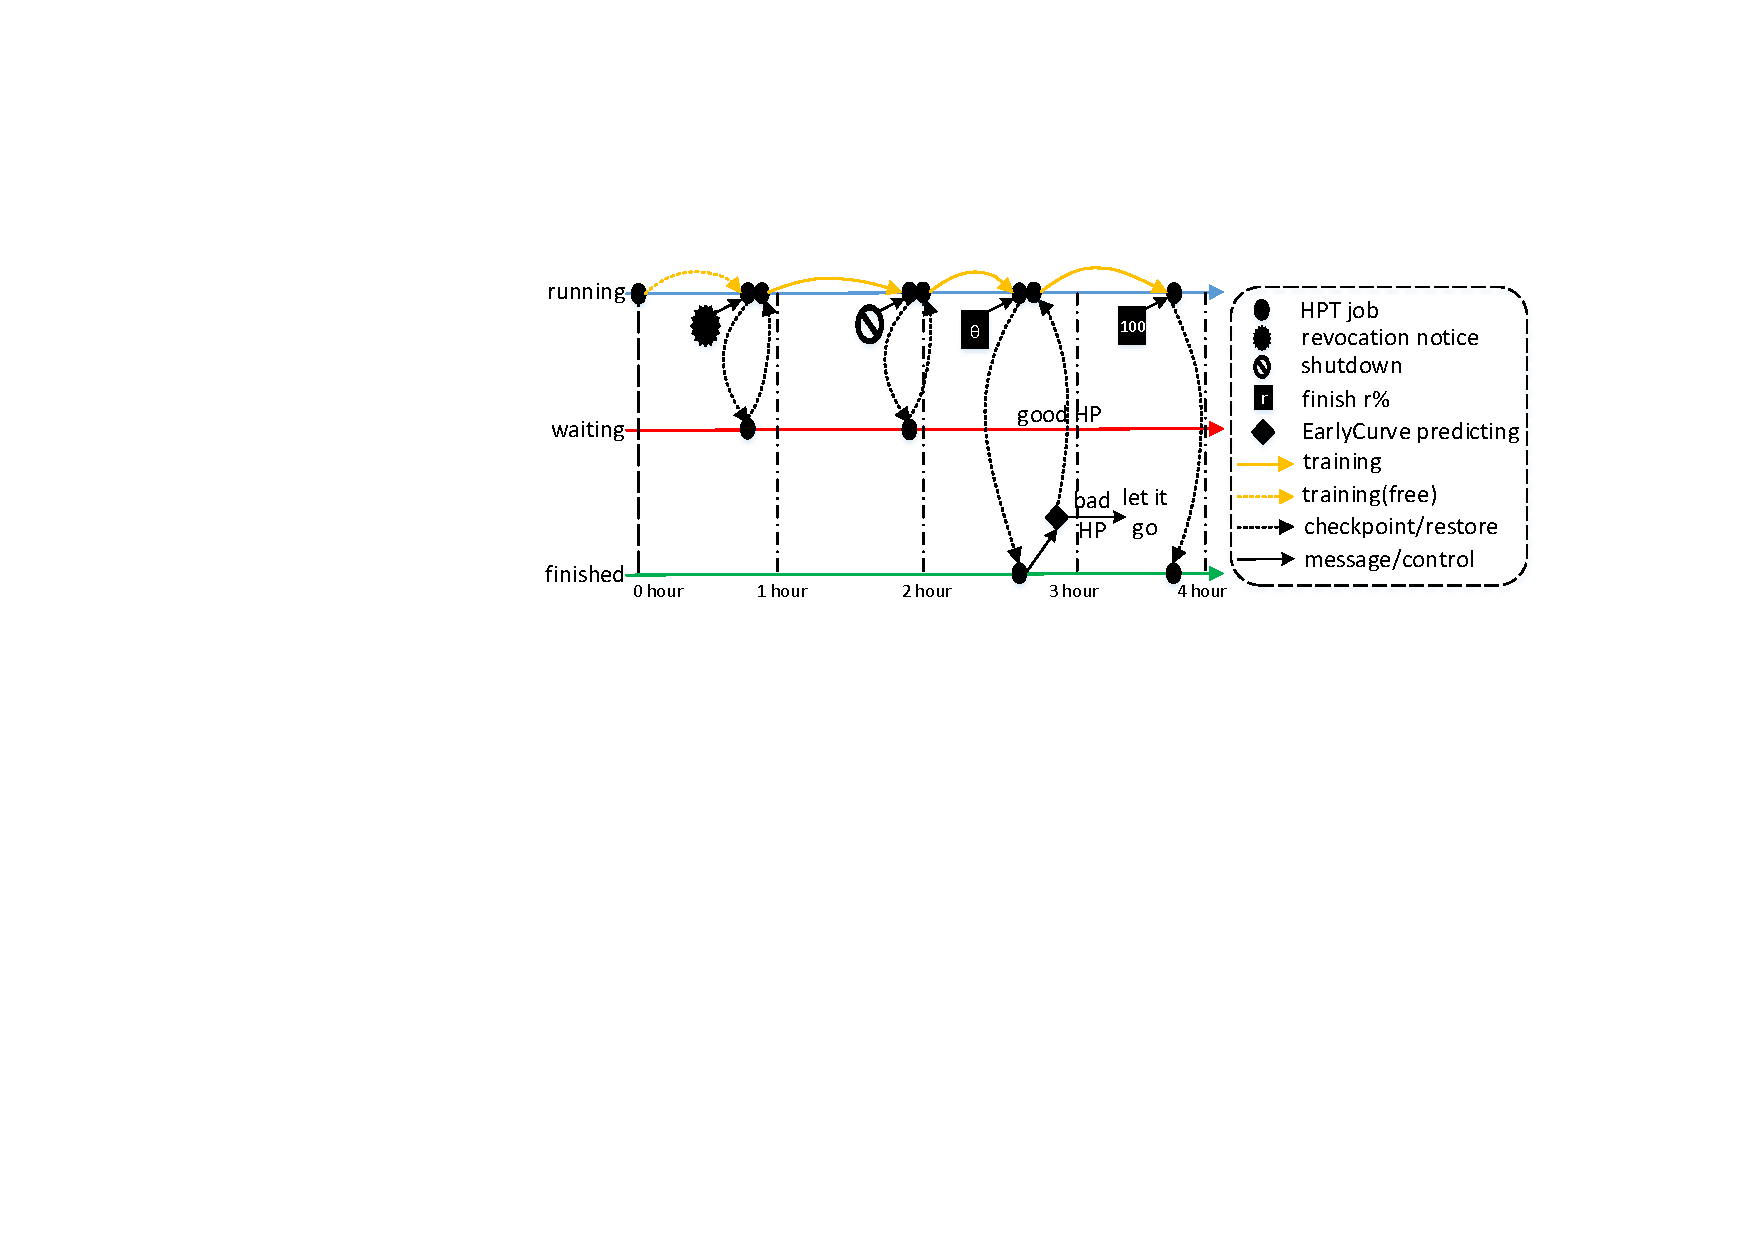
\includegraphics[width=\textwidth]{figures/example_workflow_fat_v4.pdf}}
    \caption{SpotTune工作流程示例。}
    \label{example_spottune}
\end{figure}

图~\ref{example_spottune}给出了SpotTune的一个示例工作流程。在该流程中,一个HPT任务被启动的第一小时就被回收,因此第一小时的算力对于SpotTune而言是免费的。后面该模型再次被调度之后运行超过了一小时,因此被SpotTune主动停止,并再次被调度到别的实例上。最终,当任务完成度为$\theta$时,SpotTune判断其是否是一个优秀的模型,如果是的话将继续训练直到结束,否则其占用的计算资源将被直接释放掉。

\begin{figure}[h]
    \centerline{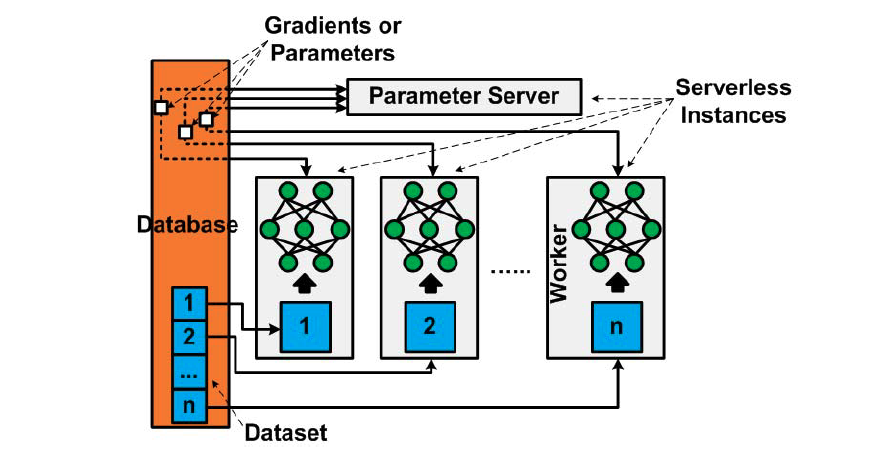
\includegraphics[width=\textwidth]{figures/data-para-faas-ml.png}}
    \caption{基于PS架构的serverless ML系统。}
    \label{data_para_faas_ml}
\end{figure}

SpotTune通过利用云上的动态资源,辅以一定的资源选取策略和ML训练过程预测算法,使得HPT可以在云上经济高效的运行。与Proteus类似,该类系统常常将成本放在系统设计的首位。云计算以其pay-as-you-go的使用模型俘获了大量用户,然而大到企业用户,小到个人用户,往往都会将成本放在首位,因为在云上获得的任何算力都会直接或间接地转化为经济开销,对于机器学习这种耗费算力的场景更是如此。正因为这样场景的普遍性存在,类似Proteus和SpotTune的基于云商服务进行二次开发的第三方系统才层出不穷。

\subsection{基于FaaS的模型训练系统}
%infocom 19
除了上述基于IaaS服务的ML系统外,近年来基于新型计算模式FaaS的ML系统也逐渐进入学术圈的视野。FaaS,亦即serverless computing,是一种新型的计算模式。其关键词serverless是一个用户维度的特征词,并非真的没有服务器,而是在用户的角度感知不到后端服务器的存在。用户只需要上传其业务代码,并声明相应的hook API,即可在云端部署一个事件驱动的function,这也是FaaS,即function as a service这一代称的由来。用户的函数一般按照请求次数收费,并且根据请求负载的变化,云厂商会进行弹性伸缩。这种细粒度的收费模式和弹性的使用模式使得应用上云变得更为简单,也自然有学者想到将其与ML联系在一起。

然而,serverless computing实际上并不是天然适用于ML系统的,要实现FaaS风格的ML系统,势必要在当前的serverless computing框架之上进行深度修改。总体而言,若要应用于ML的工作负载,serverless computing目前还存在如下问题:

\textbf{1. 本地内存和磁盘空间小。}通常而言,为了更快的横向拓展,轻量是函数计算设计的第一要义。因此,目前流行的FaaS架构,所支持的内存大小和磁盘大小都有限。例如AWS Lambda仅支持最多3GB的本地内存和512MB的本地磁盘。而现有的ML系统一般会在本地保留一份完整的数据集,并将数据集全部load到内存中以加快训练过程,这与serverless的设计原则是相违背的。当下的流行的Tensorflow,Spark等框架便无法不加修改地在AWS Lambda内运行。

\textbf{2. 带宽有限,无法进行p2p通信。}与VM相比,serverless函数一般网络带宽非常有限。例如,最大的AWS Lambda函数仅支持上线为60MBps的带宽,这与数据中心中的千兆网络,万兆网络甚至Infini-band相比是非常低的。另外,serverless computing中的函数一般是无状态的,且不同的函数之间一般无法直接通信(一个函数可以在service维度调用另一个函数的API,但是同一个service的不同函数实例一般无法感知其它函数实例的存在)。因此,在本地数据中心中常用的通信策略,例如树形或者环形的all-reduce通信在serverless环境中是无法实现的。

\textbf{3. 生命周期短且启动时间不稳定。}Serverless函数一般是为在线的service设计的,因此其生命周期天然较短。同时其启动时间不稳定,例如AWS Lambda的启动时间甚至最长可以达到一分钟。因此,基于serverless computing的ML系统必须能够很好的处理频繁的函数启停。

\textbf{4. 缺少快速的共享存储支持。}为了解决函数之间无法通信的问题,共享存储是一种常用的手段。但目前云环境中支持serverless使用的共享存储仅限于对象存储、数据库等SaaS服务,其响应延时、吞吐量等仍然无法与数据中心环境中的共享内存相比。

L. Feng等人\parencite{feng2018exploring}在2018年提出了一种简单的基于serverless的ML训练框架,其系统仍然采用PS作为主要框架。为了解决不同函数之间无法直接通信的问题,其采用云数据库作为中间存储层,使得不同的函数实例通过共享存储的方式进行通信。这一思想类似操作系统中进程间通信(IPC)的实现方式之一,即共享内存。图~\ref{data_para_faas_ml}描绘了该系统的架构图。其PS架构中的server和worker的实体都是函数。由于云数据库本身没有对参数进行聚集、更新、分发的能力,其server函数实际上负责参数的push和pull操作,数据的实际存储位置还是在数据库中。

\begin{figure}[h]
    \centerline{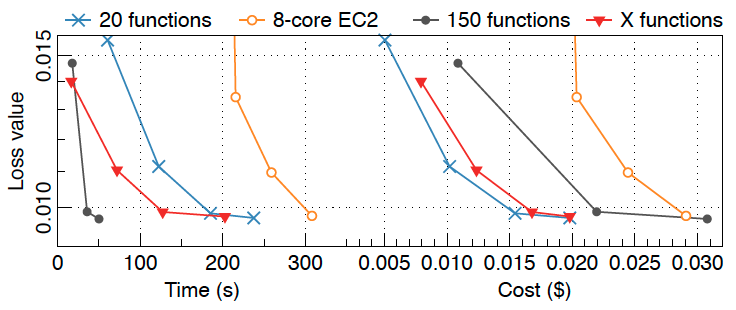
\includegraphics[width=\textwidth]{figures/ec2-lambda-diff.png}}
    \caption{在AWS Lambda和EC2上训练一个逻辑回归模型的耗时和花费。每个点代表一个epoch。}
    \label{ec2_lambda_diff}
\end{figure}

基于上述基本架构,H. Wang等人\parencite{wang2019distributed}在2019年提出了基于serverless computing的ML系统Siren,使用强化学习算法来辅助决策整个系统中的函数个数和分布。其基本假设在于,不同的函数数量会导致不同的训练完成事件和最终花费,且其模式难以通过简单的规律来总结。而且对于不同的ML模型,规律也不尽相同。图~\ref{ec2_lambda_diff}以在一个具有8核心CPU的EC2虚拟机实例上训练模型耗费的时间和产生的花费作为baseline对比了不同的函数数量下花费和耗时的不同。

\begin{figure}[h]
    \centerline{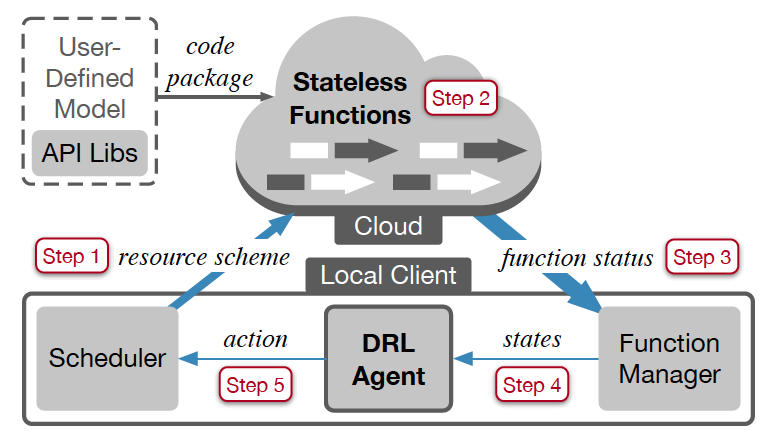
\includegraphics[width=\textwidth]{figures/siren-arch.png}}
    \caption{Siren系统架构和工作流。}
    \label{siren_arch}
\end{figure}

图~\ref{siren_arch}描述了Siren的系统架构和工作流。用户基于Siren提供的API Lib提供其模型代码包和数据集。上传至公有云之后,Siren对任务进行初始化并开始运行。运行过程中每个epoch产生的数据将反馈给Function Manager,然后Function Manager将上述数据反馈给强化学习调度器。调度器根据上述数据计算当前的reward并输出下一次决策的action,并反馈给scheduler,最终重新配置函数资源,开始下一个epoch的训练。与L. Fang等人的工作类似,Siren也采用了基于共享存储的PS架构。

事实上,serverless computing对ML的限制不仅仅在于网络通信,函数内部同样存在限制。例如,AWS Lambda中,代码包的大小被限制到250MB,运行时长被限制到300秒,运行内存大小限制到3GB。Siren采取了如下措施规避上述限制:1)重新编译MXNet,去掉USE\_CUDA,USE\_CUDNN,USE\_OPENMP等并行选项,因为serverless函数可以成千上万的并发,因此Siren追求的是函数级别的并发,而非函数内部进程级别的并发;2)每一个epoch由调度器重新分配一次函数,这与强化学习的reward-action机制也相符合。

Siren的经济高效是由其强化学习调度器所决定的。该调度器接受每个epoch结束后的函数状态作为输入设计reward函数,并进行下一次调度。图~\ref{drl_siren}展示了Siren的强化学习调度器的决策流程。关于其强化学习算法的细节设计此处不再赘述,亦非本报告所关注的重点。

\begin{figure}[h]
    \centerline{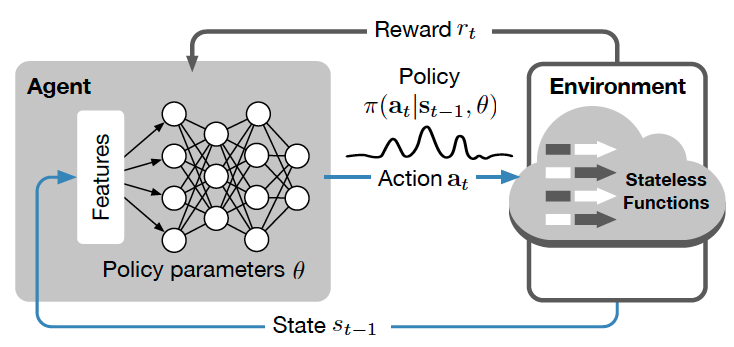
\includegraphics[width=\textwidth]{figures/drl-siren.png}}
    \caption{Siren中强化学习调度器的工作流程。}
    \label{drl_siren}
\end{figure}

整个ML模型产出的周期中不仅包含模型训练,还包括数据预处理、超参数调整等。在serverless computing的环境下支持一站式的ML工作流,如下两个问题可能会得到解决:

\textbf{1. 资源超配。}在ML的整个工作流中,资源利用率实际上变化是十分剧烈的。在以VM为计算设施的环境中,开发者为了能够性能,通常会按照整个工作流中的资源利用率峰值来配置和获取资源,这无疑造成了严重的资源浪费。而serverless computing拥有优秀的弹性,能够根据工作负载的实际强度为用户配置合适的资源,从而可能解决这类资源超配问题。

\textbf{2. 透明的资源管理。}一般而言,专业的机器学习从业人员并不具备熟练的系统配置与优化技能。因此,现有的基于VM的环境配置方案,特别是在分布式场景下,为开发人员施加了很大的压力。因此亟需一直透明的资源管理方法,对于ML从业人员而言,其只需关注模型相关的算法代码,其余应该交由系统完成, 这与serverless computing产生的初衷是类似的,serverless的计算模型有解决此类问题的天然土壤。

\begin{figure}[h]
    \centerline{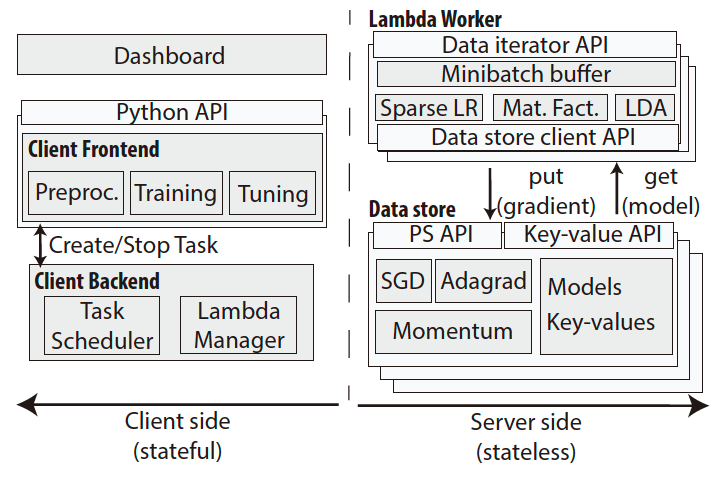
\includegraphics[width=\textwidth]{figures/cirrus-arch.png}}
    \caption{Cirrus系统架构。}
    \label{cirrus_arch}
\end{figure}

J. Carreira等人\parencite{carreira2019cirrus}在2020年提出了Cirrus,一个基于serverless的支持一站式ML工作流的框架。其支持了数据预处理、模型训练、模型调优等ML工作流中的关键阶段,并为用户提供了友好的FaaS风格的API。与前两个工作类似,Cirrus也采取PS模型作为整个系统的基础框架。图~\ref{cirrus_arch}描述了Cirrus的系统架构。所不同的是,Cirrus实现了自己的数据存储系统Data Store。

Cirrus中的Data Store是在云VM上实现的,其支持key-value的存储接口,例如set/get,和常用的PS架构接口,例如push/pull参数。其设计时通过如下几个优化,使得该存储系统实现了高并发、低延迟、高吞吐:

\textbf{1. 多线程服务器设计。}为了达到高吞吐量,Cirrus的Data Store充分利用的多线程的优势,将负载分布在不同的CPU核上。实验证明,这样的设计增加了30\%的吞吐量。

\textbf{2. 数据压缩。}为了减少网络传输的数据量,Cirrus的Data Store在get或者set时,都会将需要传输的数据进行预先压缩,这样一来所传输的数据就会大幅减少。实验证明,这样的设计将数据传输量减少了50\%。

\textbf{3. 传输稀疏数据。}Cirrus在传输参数和模型数据时,只传送那些修改了的数据条目,也就以稀疏数据的形式进行传输。实验证明,这样的设计将数据传输量进一步减少了90\%。

Cirrus屏蔽了底层设计的复杂性,向上对用户提供简洁的python接口,图~\ref{cirrus_api_example}展示了数据预处理、模型训练和超参数调整阶段Cirrus需要用户编写的代码示例。

\begin{figure}[h]
    \centerline{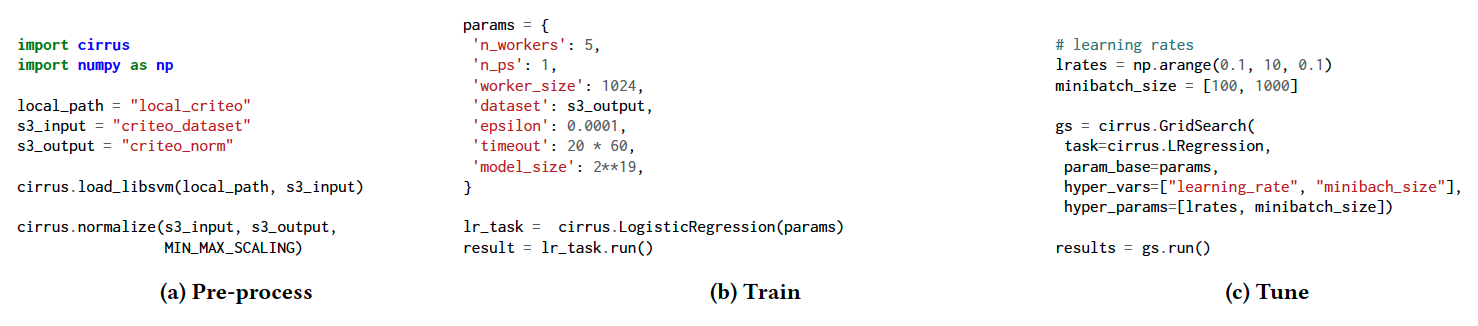
\includegraphics[width=\textwidth]{figures/cirrus-api-example.png}}
    \caption{Cirrus用户接口API示例。}
    \label{cirrus_api_example}
\end{figure}

以上述三篇工作为代表,从18-19年的架构和调度算法的优化,到20年开始研究实现serverless专用的共享存储系统,可以看出,学术界正在一步一步深入推动serverless computing在ML系统中的应用。FaaS风格的ML系统也确实解决了配置难、超配造成资源浪费等常见的问题。

\subsection{基于公有云服务的模型部署系统}
% MArk
% Tributary
在ML的工作流中,训练和调参一旦结束,就意味着产出了可以对外提供服务的模型。接下来这些模型就需要被部署到云端,为用户或者其它开发者提供服务。这类服务在日常生活和科研中是非常常见的。例如,百度提供的看图识花服务,用户只需上传一张图片,便可以得到这是何种花,甚至模型在某些情况下还会给出属于不同种类花的概率。如何将这些模型在线上部署,并且快速对用户的请求做出响应,便是模型部署系统需要解决的问题。

公有云中存在着多种多样的资源可以用来部署模型,例如IaaS和FaaS,都提供了部署模型的能力。其中IaaS中的VM还可以按照收费方式分为按需实例、预留实例和抢占实例等种类。和模型训练/调参类似,模型部署也同样需要考虑性能和成本两个角度。首先模型的在线服务也属于一种service,所以其在大多数情况下都存在对该service的质量要求,即服务等级目标(Service Level Object,SLO)。例如,一个SLO的典型例子便是要求至少95\%的请求需要在100ms内完成响应。因此,在云环境中对于模型部署系统的研究一般都集中在一个问题上,即如何在保证模型服务的SLO的前提下,尽量降低成本。

A. Harlap等人在2018年提出了服务部署系统Tributary\parencite{harlap2018tributary}。与其前作Proteus类似,Tributary也同样充分利用了云市场中的动态资源,例如AWS的Spot Instances。和Proteus类似,Tributary也采用了基于LSTM的价格预测模型,预测接下来一段时间内资源池中的所有实例在运行该服务时的潜在花费,并在其中选取最优实例。和Proteus相比,实际上是一种更为简单的场景,因为service本质上是一种无状态的负载,在动态实例启停时,无需考虑对先前状态的保存和恢复。

\begin{figure}[h]
    \centerline{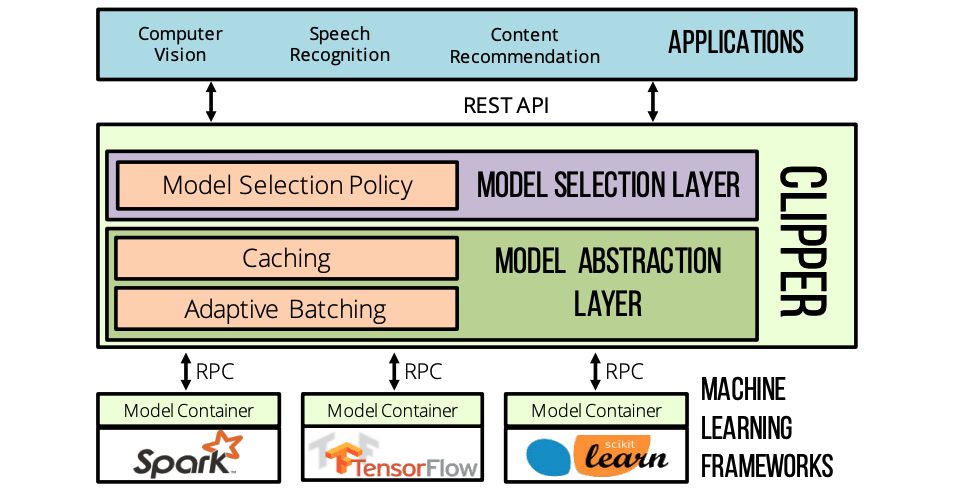
\includegraphics[width=\textwidth]{figures/clipper-arch.png}}
    \caption{Clipper系统架构图。}
    \label{clipper_arch}
\end{figure}

Tributary虽然利用云上的资源开发的模型部署系统,但仍然没有逃离传统的基于IaaS资源部署服务的模式。D. Crankshaw等人在2017年提出了Clipper\parencite{crankshaw2017clipper},一种基于容器技术的模型部署框架。如图~\ref{clipper_arch}所示,Clipper将整个部署系统抽象应用层、模型选择层、模型抽象层以及模型框架层。其向下兼容了tensorflow,spark等主流机器学习框架,向上为用户提供统一的REST API。Clipper还采用adaptive batching的技术,动态调整模型推断过程中batch size的大小,使系统的性能达到最优。

在Clipper的基础之上,C. Zhang等人在2019年提出了MArk\parencite{zhang2019mark},一种基于多种云资源混用的模型部署系统。其充分研究了公有云上不同类型资源的特点和差异性,包括常规的VM,容器服务,动态VM,突发型VM,以及GPU型VM,以便指定相应的算法,在合适的场合使用合适的资源。这里对突发型的VM实例,即Burstable Instances做简单介绍。该种类型的实例CPU能力在平时维持在一个性能较低的水平,但是用户可以令其在特定时刻以较高的性能维持一段时间。一般而言,该种类型实例的价格比按需型实例要低很多。

其经过一些列的实验,C. Zhang等人得出如下四条结论:1. 基于VM进行模型部署可以达到最优的花费和最优的性能,但是难以处理突发的增量请求。如果将其与FaaS服务相结合,或许可以解决上述问题。2. 突发型的实例可能可以应对突发的请求。3. 在按需型实例中,比较小的实例性价比更高,虽然和大型的实例相比其响应延时也要更高。4. 只有将请求进行适当的打包批量处理,才可能发挥GPU型实例的优势,使其响应延时和花费优于CPU型的实例。

基于上述四条观察,作者提出了MArk。图~\ref{mark_arch}描述了MArk的系统架构。其后端将多种云资源视作潜在的资源池,根据负载的动态变化和SLO的具体要求来进行资源选择和配置。MArk的资源配置策略可以概括为如下3条,其细节本文不再详述。

\textbf{1. 确定最佳的Batching参数。}在GPU实例上进行Batching可以达到较好的服务质量和较优的花费,但是Batching的两个重要参数,batching队列长度和batching等待时间,却需要精心调整。作者根据公式~\ref{eq_batching},辅以线下性能建模的方式,来确定最佳的参数选择。

\begin{equation}\label{eq_batching}
    \begin{aligned}
        &W_{batch} + T_b \leq RT_{max}, \\
        &W_{batch} + T_b \leq \frac{b}{\mu^*_{nb}}
    \end{aligned}
\end{equation}

\textbf{2. 使用Lambda和Burstable Instances应付突发的请求。}虽然使用VM来进行模型部署能达到最优花费和性能,但是VM的启动时间过长,在请求数量突然增多时,难以快速横向拓展来进行应对。Lambda具有较短的启动时间和较强的横向拓展能力,可以用来处理突发请求,当扩容的VM启动之后,再将流量导向新增的VM实例。同时MArk还预先启动了若干单价便宜的Burstable Instances,当请求增多时,也可以额将流量暂时导向这些实例,以利用其短暂的CPU峰值性能。具体在上述两种方案之间如何选择,就依赖于MArk根据具体的负载曲线和这两种方案产生的花费多少来进行权衡。

\begin{figure}[h]
    \centerline{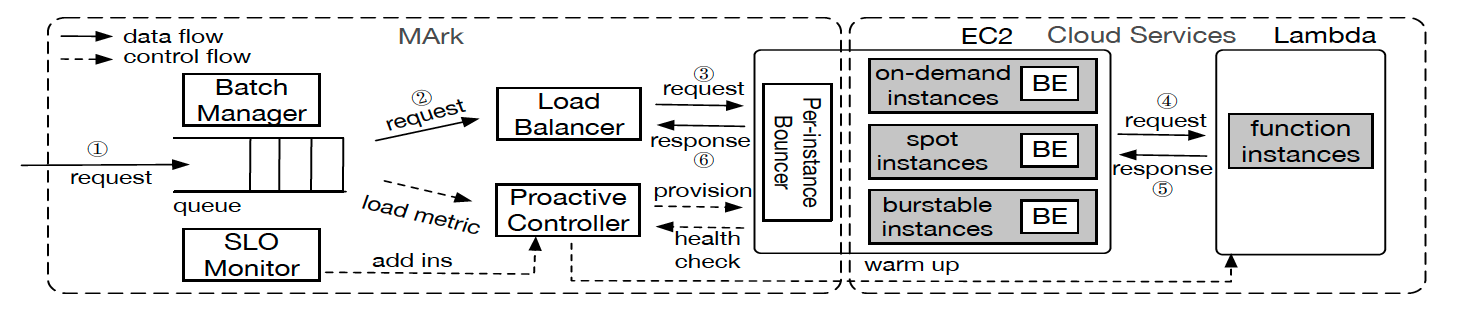
\includegraphics[width=\textwidth]{figures/mark-arch.png}}
    \caption{MArk系统架构图。}
    \label{mark_arch}
\end{figure}

\subsection{基于FaaS的模型部署系统}
%一系列FaaS for ML serving的工作,INFaaS etc
FaaS最常用的使用场景就是服务的云端部署,从这个角度来讲,不考虑serverless computing本身的若干缺点,纯FaaS的模型部署方式几乎是最理想的。尤其是从ML用户的角度而言,一旦模型完成训练和调参,用户只需将模型文件上传到云端,并声明相应的API,即可完成模型的部署,至于弹性伸缩则交由后端的云商来做即可。

\begin{figure}[h]
    \centerline{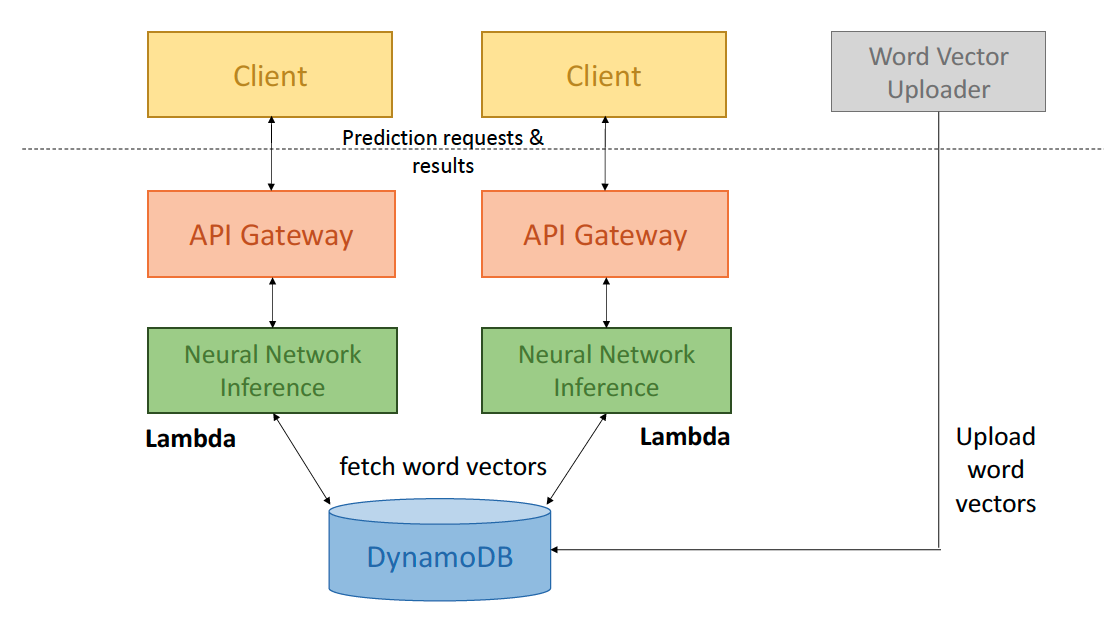
\includegraphics[width=\textwidth]{figures/nlp-serving-arch.png}}
    \caption{NLP模型在AWS云环境的部署。}
    \label{nlp_serving_arch}
\end{figure}

V. Ishakian等人\parencite{ishakian2018serving}在2018年在AWS Lambda上基于MXNet测试了若干模型对外提供服务的能力。其结论可以用一句话来概括:在热启动的前提下,利用serverless服务进行模型的在线部署是可行的,无论性能还是花费都可以接受,但是第一次请求会因为冷启动造成非常明显的高延时。Ishakian等人测试的主要是图像分类相关的模型,而Z. Tu等人\parencite{tu2018pay}在2018年针对自然语言处理的模型在AWS Lambda进行的相关实验。图~\ref{nlp_serving_arch}展示了在AWS的云环境中部署NLP模型的示例。如图所示,除了Lambda,该系统还用到了AWS的云数据库服务DynamoDB来存储词向量。模型部署之前用户先将训练得到的词向量上传至云数据库中,在实际对外提供服务时,Lambda会按需从DynamoDB中获取相关的词向量。然而在这种系统设计中仍然存在两个问题。首先,冷启动的问题仍然没有解决。其次,由于Lambda没有本地的词向量缓存,在请求频率比较高的场景下,云数据库的延时和吞吐率难以满足服务的SLO。

因此,现有的公有云上以AWS Lambda为代表的FaaS服务难以直接应用于模型部署。然而FaaS只是一种云资源的使用模式,并非于某个云厂商绑定,学术界也开始更多的探索更为先进的FaaS架构。F. Romero\parencite{romero2019infaas}等人在2019年提出INFaaS,一种model-less的模型部署系统。该模型部署系统假设用户对一个服务有两个维度的需求,即准确率和延迟。例如,某个图像识别的用户可能要求模型能够以不低于95\%的识别准确率在200ms内输出识别结果。对于不同的用户和不同的场景,这样的SLO是不尽相同的。F. Romero等人注意到,同一任务的不同模型变体在模型效果和延迟上存在很强的多样性,可能可以用来满足不同场景下的需求。例如,对于图像分类任务,VGG16和Resnet50都是常用的模型,但是两个模型在准确率和延迟方面各不相同,VGG16准确率稍低,但同时延迟也比较低,Resnet50则与相反。图~\ref{model_variants}就反映了模型的多样性。

\begin{figure}[h]
    \centerline{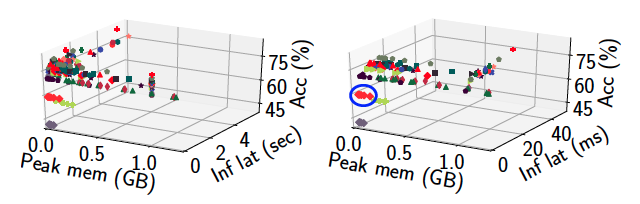
\includegraphics[width=\textwidth]{figures/model-variants.png}}
    \caption{左图为158个图像分类模型的峰值内存利用率、延迟和准确率;右图为这158个模型中延迟小于50ms的模型。}
    \label{model_variants}
\end{figure}

为了满足不同场景下用户的不同需求,F. Romero等人提出了INFaaS,根据用户的SLO要求在不同的模型变体之间进行选择并对用户的的请求做出响应。如图~\ref{infaas_arch}所示,INFaaS的工作流程如下:1)用户对前端发出请求,而后前端的Dispather根据用户的SLO需求选取当前最合适的模型,并将其反馈给worker;2)worker将模型从model repository中取出来,并派发到相应的执行器上(一般而言是CPU或者GPU)进行执行;3)模型推断结果经过前端返回给用户。Metadata Store用以存储每个模型变体的特征,例如该模型的资源消耗情况、准确率和延迟等等。Model Repository负责存储模型,在INFaas中是使用纯内存的方式实现的。同时,开发者还可以向INFaas注册和提交新的模型,提交之后的模型会先由Variant-profile对其进行采集相关特征,并存储到Metadata Store中。

\begin{figure}[h]
    \centerline{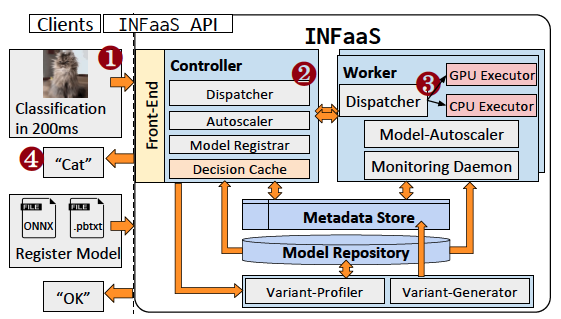
\includegraphics[width=\textwidth]{figures/infaas-arch.png}}
    \caption{INFaaS系统架构图。}
    \label{infaas_arch}
\end{figure}

值得一提的是,INFaaS称其模型部署方式为model-less的,并不意味着模型(即model)在其系统中不存在。和serverless中用户无需关注后端服务器类似,model-less意味着用户无需关注其请求到底是由系统中的那个模型变体实际为其服务的。事实上,可以认为model-less是更上一层的serverless的部署方式,因为用户不仅不需要关注后端到底存不存在服务器,甚至都不需要关注后端的模型到底是什么。

从基于云上VM,到多种服务混用,再到纯FaaS,公有云上的模型部署正在一步一步地向简洁高效发展。从云的角度理解,这是一种云原生的发展方式,即云上的模型部署依赖于云本身的能力,生在云上长在云上,将弹性伸缩、容错、高并发等工作交由云商或者第三饭服务来做,开发者或者用户只需要关注与业务本身相关的代码逻辑,即“将麻烦留给云商,将方便带给用户”。

\section{小结}
本章按照机器学习模型开发的工作流的顺序,即模型开发与调试-模型超参数调整-模型部署,介绍了面向人工智能的云计算系统软件当前的研究现状。首先介绍了公有云厂商机器学习系统的范式PS Model,以及一站式机器学习系统的代表AWS Sagemaker。Sagemaker支持从训练到部署的全部工作流程。其训练过程中使用了流行的PS Model,并为模型训练和调参设计了统一的用户API,用户只需要编写几个函数并定制几个规则即可让ML模型的训练和调参在云端自动自动展开。然而生产环境中的复杂需求也催生了一批基于云服务的第三方机器学习模型训练和调参系统,这些系统充分利用云资源类型和计费方式上的多样性,使机器学习任务在云上经济高效地运行。对于部署阶段亦是如此,模型部署方式正在经历VM-混合-FaaS的模式转变。未来基于FaaS如何对模型部署进行更好地支持,将持续成为工业界和学术界的研究热点。
% vim:ts=4:sw=4
